
%使用XeLaTeX编译
%版权所有,翻版必究
%本文件由程序自动生成,任何修改将被覆盖
%2019 年 01 月 23 日





\begin{comment}
#version 150 core
in vec2 qt_TexCoord0;
uniform float qt_Opacity;
uniform sampler2D source;
uniform float brightness;
uniform float contrast;
out vec4 fragColor;

void main() {
    vec4 pixelColor = texture(source, qt_TexCoord0);
    pixelColor.rgb /= max(1.0/256.0, pixelColor.a);
    float c = 1.0 + contrast;
    float contrastGainFactor = 1.0 + c * c * c * c * step(0.0, contrast);
    pixelColor.rgb = ((pixelColor.rgb - 0.5) * (contrastGainFactor * contrast + 1.0)) + 0.5;
    pixelColor.rgb = mix(pixelColor.rgb, vec3(step(0.0, brightness)), abs(brightness));
    fragColor = vec4(pixelColor.rgb * pixelColor.a, pixelColor.a) * qt_Opacity;
}
\end{comment}


\FloatBarrier
\section{
BrightnessContrast
}\label{c000015s000003}



%使用XeLaTeX编译
%版权所有,翻版必究
%本文件由程序自动生成,任何修改将被覆盖
%2019 年 01 月 23 日



%表
\begin{longtable}{ccc}

%表头....
\toprule{}类名 
&
分类
&
简介%there must use marginnote ...
\marginnote{\setlength\fboxsep{2pt}\fbox{\footnotesize{\kaishu\tablename\,}\footnotesize{\ref{tb000000}}}}
\\ \midrule 
\endfirsthead

%表尾...
\bottomrule
\caption{ThresholdMask}\label{tb000000} 
\endlastfoot

%重复表头
\toprule{}类名 
&
分类
&
简介
\\ \midrule
\endhead
%重复表尾
\midrule
\endfoot 
Blend & aabbc & cccc \\
BrightnessContrast & aabbc & cccc \\
ColorOverlay & aabbc & cccc \\
Colorize & aabbc & cccc \\
Desaturate & aabbc & cccc \\
GammaAdjust & aabbc & cccc \\
HueSaturation & aabbc & cccc \\
LevelAdjust & aabbc & cccc \\
ConicalGradient & aabbc & cccc \\
LinearGradient & aabbc & cccc \\
RadialGradient & aabbc & cccc \\
Displace & aabbc & cccc \\
DropShadow & aabbc & cccc \\
InnerShadow & aabbc & cccc \\
FastBlur & aabbc & cccc \\
GaussianBlur & aabbc & cccc \\
MaskedBlur & aabbc & cccc \\
RecursiveBlur & aabbc & cccc \\
DirectionalBlur & aabbc & cccc \\
RadialBlur & aabbc & cccc \\
ZoomBlur & aabbc & cccc \\
Glow & aabbc & cccc \\
RectangularGlow & aabbc & cccc \\
OpacityMask & aabbc & cccc \\
ThresholdMask  & aabbc & cccc \\
\end{longtable}
%表





%使用XeLaTeX编译
%版权所有,翻版必究
%本文件由程序自动生成,任何修改将被覆盖
%2019 年 01 月 23 日





%begin图片
\begin{figure}[htb] %浮动体 here and top ...
%there must use marginnote ...
\marginnote{\setlength\fboxsep{2pt}\fbox{\footnotesize{\kaishu\figurename\,}\footnotesize{\ref{p000019}}}}\centering %中心对齐
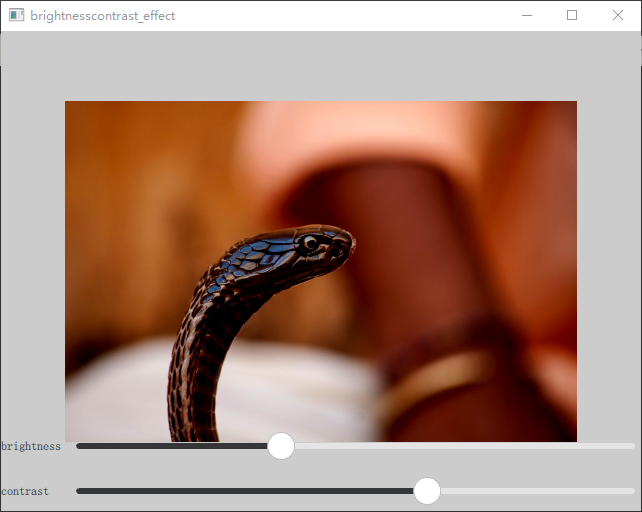
\includegraphics[width=0.95\textwidth]{../chapter06/brightnesscontrast_effect/the_app.png} %图片路径
\caption{BrightnessContrast} %标题
\label{p000019} %索引
\end{figure}
%end图片


%\begin{spacing}{1.0}
\refstepcounter{filesourcenumber}\label{f000053}    %增加源代码编号
\FloatBarrier                                  %强制完成浮动体布局
\begin{thebookfilesourceone}[escapeinside={(*@}{@*)},
caption=GoodLuck,
title=\filesourcenumbernameone \thefilesourcenumber
]
/*brightnesscontrast_effect/main.qml*/
import QtQuick 2.9
import QtGraphicalEffects 1.12

Rectangle {

    id : idRoot
    width: 640;
    height: 480;
    color: Qt.rgba(0.8,0.8,0.8,1);


    Image{
        width: parent.width * 0.8;
        height: parent.height * 0.8;
        anchors.centerIn: parent
        source: "image.jpg"
        visible: false
        fillMode: Image.PreserveAspectFit
        id : idImage
    }

    BrightnessContrast{
        anchors.fill: idImage
        source: idImage
        contrast: idControl.contrastItem.value
        brightness: idControl.brightnessItem.value
    }

    BrightnessContrastControl{
        id:idControl
    }

}(*@\marginpar[\hfill\setlength\fboxsep{2pt}\fbox{\footnotesize{\kaishu\parbox{1em}{\setlength{\baselineskip}{2pt}\filesourcenumbernameone}}\footnotesize{\thefilesourcenumber}}]{\setlength\fboxsep{2pt}\fbox{\footnotesize{\kaishu\parbox{1em}{\setlength{\baselineskip}{2pt}\filesourcenumbernameone}}\footnotesize{\thefilesourcenumber}}}@*)\end{thebookfilesourceone}          %抄录环境
\addtocounter{lstlisting}{-1}   %sub lstlisting counter ...
%\end{spacing}


%\begin{spacing}{1.0}
\refstepcounter{filesourcenumber}\label{f000077}    %增加源代码编号
\FloatBarrier                                  %强制完成浮动体布局
\begin{thebookfilesourceone}[escapeinside={(*@}{@*)},
caption=GoodLuck,
title=\filesourcenumbernameone \thefilesourcenumber
]
#version 150 core
in vec2 qt_TexCoord0;
uniform float qt_Opacity;
uniform sampler2D source;
uniform float brightness;
uniform float contrast;
out vec4 fragColor;

void main() {
    vec4 pixelColor = texture(source, qt_TexCoord0);
    pixelColor.rgb /= max(1.0/256.0, pixelColor.a);
    float c = 1.0 + contrast;
    float contrastGainFactor = 1.0 + c * c * c * c * step(0.0, contrast);
    pixelColor.rgb = ((pixelColor.rgb - 0.5) * (contrastGainFactor * contrast + 1.0)) + 0.5;
    pixelColor.rgb = mix(pixelColor.rgb, vec3(step(0.0, brightness)), abs(brightness));
    fragColor = vec4(pixelColor.rgb * pixelColor.a, pixelColor.a) * qt_Opacity;
}(*@\marginpar[\hfill\setlength\fboxsep{2pt}\fbox{\footnotesize{\kaishu\parbox{1em}{\setlength{\baselineskip}{2pt}\filesourcenumbernameone}}\footnotesize{\thefilesourcenumber}}]{\setlength\fboxsep{2pt}\fbox{\footnotesize{\kaishu\parbox{1em}{\setlength{\baselineskip}{2pt}\filesourcenumbernameone}}\footnotesize{\thefilesourcenumber}}}@*)\end{thebookfilesourceone}          %抄录环境
\addtocounter{lstlisting}{-1}   %sub lstlisting counter ...
%\end{spacing}

























%使用XeLaTeX编译
%版权所有,翻版必究
%本文件由程序自动生成,任何修改将被覆盖
%2019 年 01 月 23 日



